\chapter{Robotic arm kinematic Analysis}


\section{Robotic arm, D-H parameters \& Forward Kinematics}

The Forward Kinematics (FK) problem seeks to specify the transformations between every pair of consecutive robot links. The four\textbf{Denavit-Hartenberg} (D-H) parameters can describe the kinematic chain. Two of these parameters describe the link itself and the other two describe the link's relation to the neighboring link.
%
\begin{itemize}
\item The \textbf{length} $L_i$ of the i-th link is equal to the distance between the axes $z_i$ and $z_{i+1}$
\item The \textbf{twist angle} $α_i$ of the i-th link, is the angle between the axes $z_i$ and $z_{i+1}$
\item The \textbf{rotation angle} $θ_i$ of the link $\left\lbrace i \right\rbrace $ with respect to the $\left\lbrace i-1 \right\rbrace$ link, is the angle 
between the axes $x_{i-1}$ and $x_i$
\item The \textbf{distance} $d_i$ of the link $\left\lbrace i \right\rbrace$ with respect to the $\left\lbrace i-1 \right\rbrace$ link, is the distance 
between the axes $x_{i-1}$ and $x_i$
\end{itemize}
\begin{table}[htbp]
\begin{center}
\begin{tabular}{ |c|c|c|c|c| } 
\hline
$i$ & $θ_i$ (rad) & $L_{i-1}$ (m) & $d_i$ (m) & $α_{i-1}$ (rad) \\
\hline
1 & $θ_1$ & 0 & 0.36 & 0 \\
2 & $θ_2$ & 0 & 0 & $-π/2$ \\
3 & $θ_3$ & 0 & 0.36 & $π/2$ \\
4 & $θ_4$ & 0 & 0 & $π/2$\\
5 & $θ_5$ & 0 & 0.4 & $-π/2$ \\
6 & $θ_6$ & 0 & 0 & $-π/2$ \\
7 & $θ_7$ & 0 & 0 & $π/2$ \\
\hline
\end{tabular}
\end{center}
\caption{D-H parameters for Kuka iiwa14}
\end{table}

\begin{figure}[htbp]
\centering
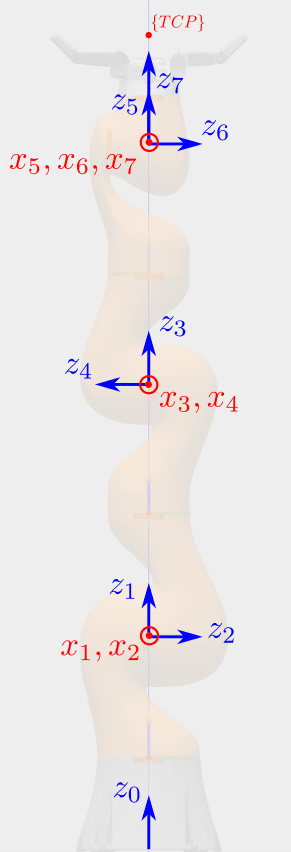
\includegraphics[height=10cm]{images/iiwa-frames.png}\\
\caption{Joint reference frames of the KUKA iiwa14 robot}
\end{figure}


The goal of the FK-problem is to find the transformation of the reference frame of the end-effector with respect to the universal reference frame. To achieve that, we must first calculate the transformations between each pair of joints. To simplify each such transformation, i.e. the transformation from a frame $\left\lbrace i-1 \right\rbrace$ to a frame $\left\lbrace i \right\rbrace$, we consider 3 intermediary reference frames $\left\lbrace A \right\rbrace$, $\left\lbrace B \right\rbrace$ and $\left\lbrace C \right\rbrace$. Then the transformations between the two joints is given by
\begin{comment}
\begin{equation}
^{i-1}T_i = ^{i-1}T_C \cdot ^{C}T_B \cdot ^{B}T_A \cdot ^{A}T_i
\end{equation}

The matrix $^{A}T_i$ expresses the translation of the coordinate system $\left\lbrace i \right\rbrace$ with respect to $\left\lbrace A \right\rbrace$ by a distance $d_i$ along the axis $z_i$
\begin{equation}
^{A}T_i = 
\begin{bmatrix}
1 & 0 & 0 & 0\\
0 & 1 & 0 & 0\\
0 & 0 & 1 & d_i\\
0 & 0 & 0 & 1\\
\end{bmatrix}
\end{equation}

The matrix $^{B}T_A$ expresses the rotation of the coordinate system $\left\lbrace A \right\rbrace$ with respect to $\left\lbrace B \right\rbrace$ by an angle $θ_i$ around the axis $z_i$
\begin{equation}
^{B}T_A = 
\begin{bmatrix}
c\theta_i & -s\theta_i & 0 & 0\\
s\theta_i & c\theta_i & 0 & 0\\
0 & 0 & 1 & 0\\
0 & 0 & 0 & 1\\
\end{bmatrix}
\end{equation}

The matrix $^{C}T_B$ expresses the translation of the coordinate system $\left\lbrace B \right\rbrace$ with respect to $\left\lbrace C \right\rbrace$ by a distance $L_{i-1}$ along the axis $x_{i-1}$
\begin{equation}
^{C}T_B = 
\begin{bmatrix}
1 & 0 & 0 & L_{i-1}\\
0 & 1 & 0 & 0\\
0 & 0 & 1 & 0\\
0 & 0 & 0 & 1\\
\end{bmatrix}
\end{equation}

The matrix $^{i-1}T_C$ expresses the rotation of the coordinate system $\left\lbrace C \right\rbrace$ with respect to $\left\lbrace i-1 \right\rbrace$ by an angle $a_{i-1}$ around the axis $x_{i-1}$
\begin{equation}
^{i-1}T_C = 
\begin{bmatrix}
1 & 0 & 0 & L_{i-1}\\
0 & ca_{i-1} & -sa_{i-1} & 0\\
0 & sa_{i-1} & ca_{i-1} & 0\\
0 & 0 & 0 & 1\\
\end{bmatrix}
\end{equation}

Using the D-H parameters of the aforementioned table and the product of the above 4 matrices, one can calculate the transformation matrix between two consecutive links, and is calculated as the following
\end{comment}
\begin{equation}
^{i-1}T_i = 
\begin{bmatrix}
c\theta_i & -s\theta_i & 0 & L_{i-1} \\
s\theta_ica_{i-1} & c\theta_ica_{i-1} & -sa_{i-1} & -sa_{i-1}d_i \\
s\theta_isa_{i-1} & c\theta_isa_{i-1} & ca_{i-1} & ca_{i-1}d_i \\
0 & 0 & 0 & 1\\
\end{bmatrix},
\end{equation}
where $c\theta_i = \cos(\theta_i),~s\theta_i=\sin(\theta_i), sa_i=\sin(a_i)$ and $ca_i=\cos(a_i)$.

The total transformation $^{0}T_N$, which represents the position and the 
orientation of the local coordinate system of the end-effector with respect to the global coordinate system of the robot's base can be found by 
\begin{equation}
^{0}T_N = {}^{0}T_1 \cdot {}^{1}T_0 \cdots {}^{N-1}T_N.
\end{equation}
The orientation is the upper-left $3\times3$ matrix and the position is given by the fourth column of the matrix $^{0}T_N$.

\begin{comment}
All transformations $^{i-1}T_i$ are members of a special set of matrices (Lie Group), called \textbf{Special Euclidean Group}
\[
^{i-1}T_i \in SE(3) = \left\lbrace \begin{bmatrix}
R & \mathbf{p}\\
\mathbf{0} & 1
\end{bmatrix} : R \in SO(3), \mathbf{p} \in \mathbb{R}^{3} \right\rbrace
\]
where $SO(3)$ is another Lie Group called \textbf{Special Orthogonal Group}
\[
SO(3) = \left\lbrace R \in \mathbb{R}^{3 \times 3}: R^{-1}=R^\top, det(R)=1 \right\rbrace
\]

The properties of $SE(3)$ and $SO(3)$ are very useful in all the calculations of various transformations because it can reduce the amount of matrix operations and also speeds up the calculation 
of inverse matrices.
\end{comment}
The workspace of the robot arm is the set of all points in $\mathbb{R}^3$ that the tip of the manipulator can reach.
\begin{figure}[htbp]
\centering
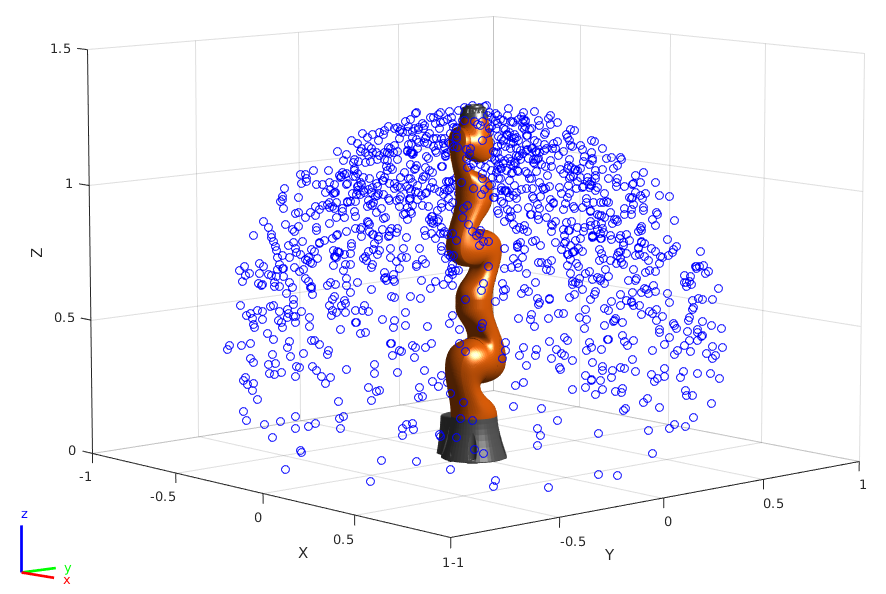
\includegraphics[width=0.5\textwidth]{images/workspace_sampling_1e3.png}\\
\caption{KUKA iiwa14 workspace calculated with FK by randomly sampling the value ranges of the joints.}
\end{figure}

\subsection{End-effector to tool-tip transformations}
\label{section:eef-tool-tip-transformations}

The surgical tool is attached to the end-effector of the arm; the corresponding frames are in agreement with the drawing shown in Figure~\ref{fig:kuka-surgical tool}. 
The corresponding transformations can be found as
\begin{equation*}
^{7}T_{TCP} = 
\begin{bmatrix}
1 & 0 & 0 & 0 \\
0 & 1 & 0 & 0 \\
0 & 0 & 1 & 0.094 \\
0 & 0 & 0 & 1 \\
\end{bmatrix}
,
^{TCP}T_{B} = 
\begin{bmatrix}
1 & 0 & 0 & 0.05 \\
0 & 0 & -1 & 0 \\
0 & 1 & 0 & 0 \\
0 & 0 & 0 & 1 \\
\end{bmatrix}
,
^{B}T_T = 
\begin{bmatrix}
1 & 0 & 0 & -0.01 \\
0 & 1 & 0 & 0.022 \\
0 & 0 & 1 & 0.455 \\
0 & 0 & 0 & 1 \\
\end{bmatrix}
\end{equation*}

\begin{figure}[htbp]
\centering
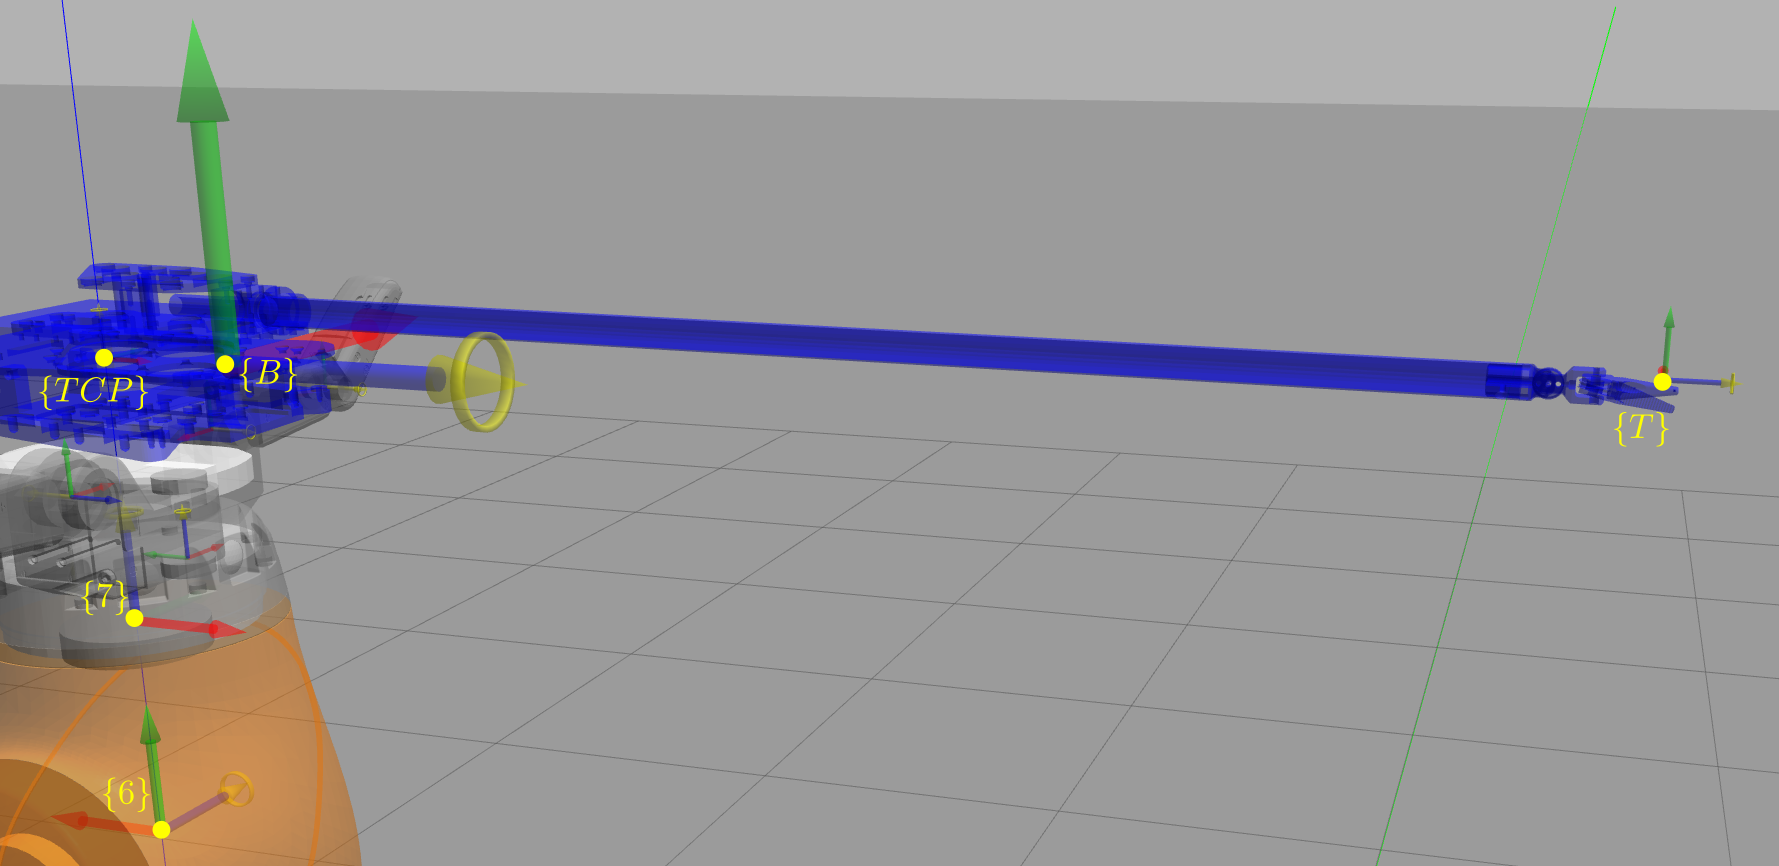
\includegraphics[width=0.8\textwidth]{images/eef_tcp_tip_tf.png}\\
\caption{Reference frames of last link $\lbrace 7 \rbrace$, end-effector $\lbrace TCP \rbrace$, surgical tool base (center of mass) $\lbrace B \rbrace$ and tool-tip frame $\lbrace T \rbrace$}
\label{fig:kuka-surgical tool}
\end{figure}

\section{Inverse Kinematics}

The Inverse Kinematics (IK) problem seeks to find those joint values that make the robot's end effector to be at a specific desired position and orientation. For a robot with more Degrees of Freedom (DoF) than the demanded six to fully position and orient a robot in 3D space (3 for position and 3 for orientation), the IK has infinite solutions. Thus an additional constraint is required to find a specific solution. This extra degree of freedom is very useful in finding kinematic solutions that are optimal under some circumstances and are also useful in avoiding \textbf{singularity points}.

\subsection{Decoupling Technique}

In this section the inverse kinematics problem is solved for 6 out of the 7 DoF, where the third joint is not used in this analysis and its angle is set to zero $θ_3 = 0$ . Using the decupling technique, the IK-problem is split to 2 separate subproblems, one for the position and one for the orientation of the end-effector. This technique can be applied in this case because the axes of the 3 last joints intersect at the same point and they form an Euler wrist. 

To solve for the joints' angles, the transformation matrix $^0T_7$ of the end-effector with respect to the robot's base is required. Usually the transformation ${}^UT_{tcp}$ is known, which is the pose of Tool's center point (TCP) with respect to the Universal Coordinate Frame $\lbrace U \rbrace$ from which the required $^0T_7$ can be calculated

\begin{equation}
{}^UT_{TCP} = {}^UT_0  \;  {}^0T_7  \;   {}^7T_{TCP}
,
~
{}^0T_7 = {}^UT_0^{-1}  \;\;  {}^UT_{TCP}  \;\;  {}^7T_{TCP}^{-1}
,
~
{}^0T_7 = \begin{bmatrix}
R_t & \mathbf{p}_t \\
0 & 1 \\
\end{bmatrix}
\end{equation}
%
where ${}^UT_0,  \;\;   {}^7T_{tcp}$ are translation transformations by a constant distance and $R_t,  \;\; \mathbf{p}_t$ are the target's orientation 
and position respectively.

Simple geometric principles can be used to infer the relationships for all angles.
\begin{center}
\begin{figure}[htbp]
\centering
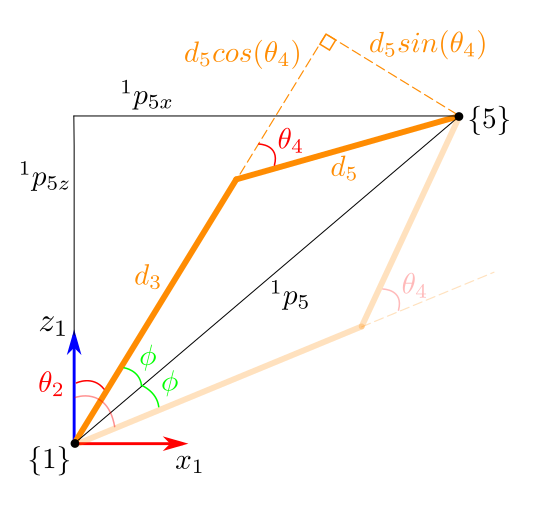
\includegraphics[width=6cm]{images/th2-4-calculation.png}\\
\caption{Calculation of angles $θ_2, θ_4$}
\label{iiwa14-solution-configurations}
\end{figure}
\end{center}

\begin{eqnarray}
{}^0\mathbf{p}_5 &=& {}^0T_4 {}^4\mathbf{p}_5 = \begin{bmatrix} p_x \\ p_y \\ p_z \\ \end{bmatrix}
\\
θ_1 &=& 
\begin{cases}
atan2 \left( p_y, p_x \right) \\
π - atan2 \left( p_y, p_x \right)
\end{cases}
\\
φ &=& acos \left( \frac{d_3^2 + \Vert{}^1p_{5}\Vert ^2 - d_5^2}{2d_3 \Vert{}^1p_{5}\Vert} \right),
~
θ_2 = atan2 \left( \sqrt{p_x^2 + p_y^2}, {}^1p_{5z} \right) \pm φ
\\
c_4 &=& \frac{ \Vert{}^1p_{5}\Vert ^2 - d_3^2 - d_5^2 }{2d_3d_5},~
θ_4 = atan2 \left( \pm \sqrt{1 - c_4^2}, c_4 \right)
\end{eqnarray}
Having computed $\theta_i,~i=1,\ldots,4$, the orientation matrix of the wrist can be calculated as following
\begin{eqnarray}
R_{target} &=& 
\begin{bmatrix}
i_x & j_x & k_x\\
i_y & j_y & k_y\\
i_z & j_z & k_z\\
\end{bmatrix}
\nonumber
\\
θ_6 &=& atan2 \left( \pm \sqrt{1-k_y^2}, k_y \right)
\\
θ_7 &=& atan2 \left( -j_y, i_y \right)
\\
θ_5 &=& atan2 \left( - k_z, k_x \right)
\end{eqnarray}

\begin{center}
\begin{figure}[!htb]
\centering
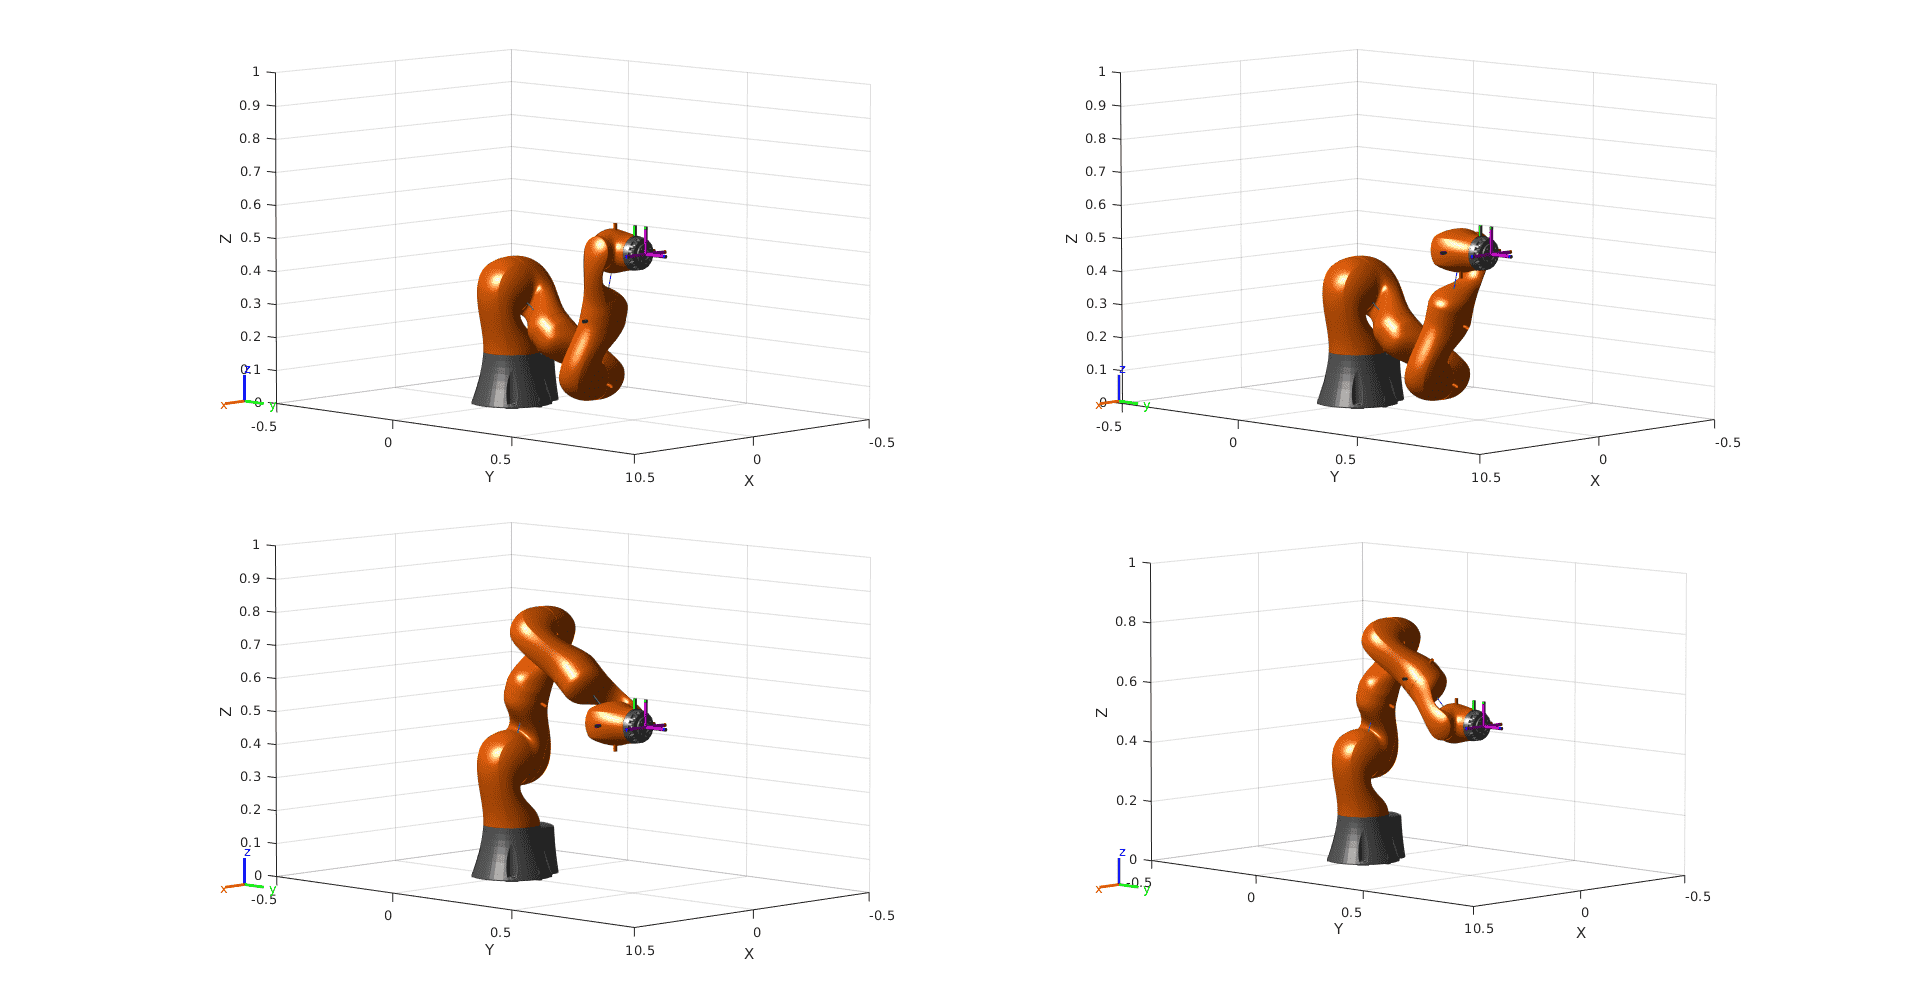
\includegraphics[width=0.8\textwidth]{images/ik-4-solutions.png}\\
\caption{The first 4 out of 8 solutions of the IK-problem}
\end{figure}
\end{center}

\subsection{Numerical solutions for 7 DoF robot arm}

Tand the joint derivatives. These two vectors are related by a matrix known as the 
The \textbf{Jacobian} of the manipulator is 
\begin{equation}
\mathbf{\dot{x}} = J( \mathbf{q} ) \mathbf{\dot{q}} =
\begin{bmatrix}
\dfrac{\partial \mathbf{f}_1(\mathbf{q})}{\partial q_{1}} & \cdots & \dfrac{\partial \mathbf{f}_1(\mathbf{q})}{\partial q_{7}} \\
\vdots & \ddots & \vdots \\
\dfrac{\partial \mathbf{f}_6(\mathbf{q})}{\partial q_{1}} & \cdots & \dfrac{\partial \mathbf{f}_6(\mathbf{q})}{\partial q_{7}} \\
\end{bmatrix} 
\mathbf{\dot{q}},
\end{equation}
where $\mathbf{x} \in \mathbb{R}^6$ is the position and orientation of the robot's end-effector and $\mathbf{q} =\left[ \theta_1,\ldots,\theta_7\right]^{\top} \in \mathbb{R}^7$; in the sequel rather than using $\theta_i$ the adopted symbol $q_i$ is selected.

$J( \mathbf{q} )$ is non rectangular owing to the additional 7th DoF and its pseudoinverse is computed as $J^{\dagger} = J^\top ( J J^\top )^{-1}$. Then a sequential algorithm is used to compute $\mathbf{q}$, as
\begin{algorithm}[H]
\SetAlgoLined
initialize $\mathbf{q}^0 \in \mathbb{R}^{7}$ with an initial guess, given a desired position and orientation $\mathbf{x}_d \in \mathbb{R}^{6}$\;
set error $e = \mathbf{x}_d - f(\mathbf{q^i})$\;
set error tolerance $ε$ with some small value\;
\While{$e \geq ε$}{
	set $\mathbf{q}^{i+1} = \mathbf{q}^i + J^{\dagger}( \mathbf{q} )e$\;
	$i \leftarrow i + 1$\;
}
\caption{Newton-Raphson numerical method for computing $\mathbf{q}$.}
\end{algorithm}

The convergence to local minima needs attention and a recursive form that uses the previously computed solution to the 6 DoFs is used to provide $\theta_i,~i\in\{ 1,\ldots,7\}/3$.

The columns of the Jacobian matrix are 
\begin{comment}
\[
J_v = J_v( \mathbf{q} ) = [ J_{v1}, J_{v2}, \cdots, J_{v7} ] \in \mathbb{R}^{6 \times 7}
\]
\end{comment}
\begin{equation}
J_i = \begin{bmatrix}
{}^0\mathbf{z}_i \times ({}^0\mathbf{p}_8 - {}^0\mathbf{p}_i) \\
{}^0\mathbf{z}_i \\
\end{bmatrix},~i=1,\ldots,7.
\end{equation}


\subsection{Constraints \& Singularity points}
%
\subsubsection{Workspace constraints \& Singularity points}
%
When studying the kinematics of a robotic arm it is important to study the singularity points, which must be known before path planning in order to be avoided. From a mathematical point of view, singularity points are defined as these spatial joint coordinates where the kinematics equations are not defined, e.g. when dividing by a quantity that becomes zero or is very close to zero or when the determinant of the robot's Jacobian approaches zero (as shown in Figure~\ref{robot-planner1-manipulability-plot}), or even when the inverse kinematics solutions are infinite. 

Singularity points typically reduce the kinematic capability of the robot. An example of that are points where the end-effector cannot move at all or it cannot move in some directions. An other example of singularity points, are those in which small displacements/velocities in the taskspace require very large displacements/velocities in the joint space and sometimes with velocities much higher than the rated values of the actuators

For the Kuka iiwa 7 DoF arm, the singularity points are:
\begin{itemize}
	\item When $p_x^2 + p_y^2 = 0$ then the end-effector lies on the z-axis and $θ_1$ is not defined
	\item When the axes $z_1,z_7$ coincide, then $θ_1,θ_7$ can no longer be defined
	\item When $\sin\left( θ_6 \right) = 0$ then the angles $θ_5, θ_7$ are not defined. According to the robot's manual and the equations of inverse kinematics above, there are an infinite number of combinations of
	$θ_5, θ_7$ to get the same position on the end-effector.
	\item When the shoulder is fully extended, $θ_1$ and $θ_3$ are not defined (there are infinite combinations for the same result)
\end{itemize}
Other kinematic singularities that are explained in more details in KUKA's Sunrise.OS 1.11 manual are the following:
\begin{itemize}
	\item Extended position $θ_4 = 0$: motion is blocked in the direction of $z_3$ and $z_5$ axes
	\item When $θ_4 = \frac{π}{2}$ and $θ_6 = 0$ the motion parallel to $z_6$ or $z_2$ is blocked
	\item When $θ_2 = 0$ and $θ_3 = \pm \frac{π}{2}$ the the motion is blocked in the direction of the robot or parallel to axes $z_2,z_5$
	\item When $θ_5 = \frac{π}{2}$ and $θ_6 = 0$ the motion parallel to axis $z_6$ is blocked
\end{itemize}
The workspace of the Kuka iiwa LBR14 is shown in the sequel taking into account the allowable region of the joint coordinates

\begin{figure}[htbp]
\centering
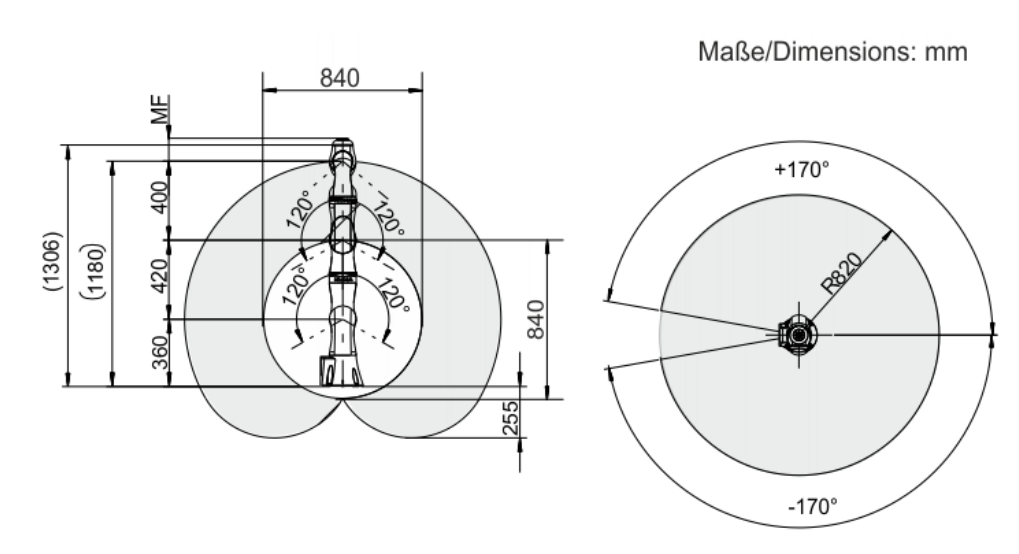
\includegraphics[width=10cm]{images/iiwa-workspace.png}\\
\caption{KUKA iiwa LBR14 workspace}
\end{figure}

\subsubsection{Remote Center of Motion constraint}
\label{rcm-subsubsection}

The Remote Center of Motion (RCM) constraint is encountered frequently in MIS. The RCM point, also known in the bibliography as fulcrum point, trocar point, incision point and/or insertion point, is a virtual point in space around which the robot is constrained to rotate (pivot). The RCM constraint means that at all times one point along the axis of the surgical tool must coincide with the RCM point. This constraint reduces the number of degrees of freedom from 6 (position and orientation in Cartesian 3D space) to only four:
\begin{enumerate}
\item \textbf{insertion} and \textbf{retraction}: translation along the $\mathbf{\hat{r}}$ vector of the spherical coordinate system of the Fulcrum Reference frame
\item \textbf{roll}, also known as pan: rotation around the $\mathbf{\hat{z}}$ unit vector by an angle $\phi$
\item \textbf{pitch}, also known as tilt: rotation around the $\mathbf{\hat{y}}$ unit vector by an angle $\theta$
\item \textbf{yaw}, also known as spin: rotation around the $\mathbf{\hat{x}}$ unit vector by an angle $\psi$
\end{enumerate}
The RCM constraint does not have a direct implication in the solutions of the inverse kinematics solution, because it only reduces the taskspace to a very specific subspace and a very specific set of robot positions and orientations.

To satisfy the RCM constraint many MIS robots have special mechanical structures that make it easier for the laparoscopic tools to pivot around the fulcrum point. The most common examples of these types of mechanisms are parallelograms, spherical linkages and circular tracking arcs, all of which have usually 2 RCM DoF. Other types of RCM mechanisms are isocenters, synchronous belt transmission, parallel manipulators, passive RCMs and compliant mechanisms~\cite{dai2009HIstoricalMISKinematicsRCM}. 
\begin{comment}In the simulation setup of this thesis there is no special RCM mechanism to satisfy the RCM constraint. A typical industrial robot arm is used and the RCM constraint is satisfied by calculating at each time the correct pose the robot must have which is used as input to the Inverse Kinematics problem. To achieve this, the RCM point must be known beforehand (or be estimated) and then all RCM poses are calculated using a spherical coordinate system, whose origin 
of axes is the RCM point.
\end{comment}
\begin{figure}[htbp]
\centering
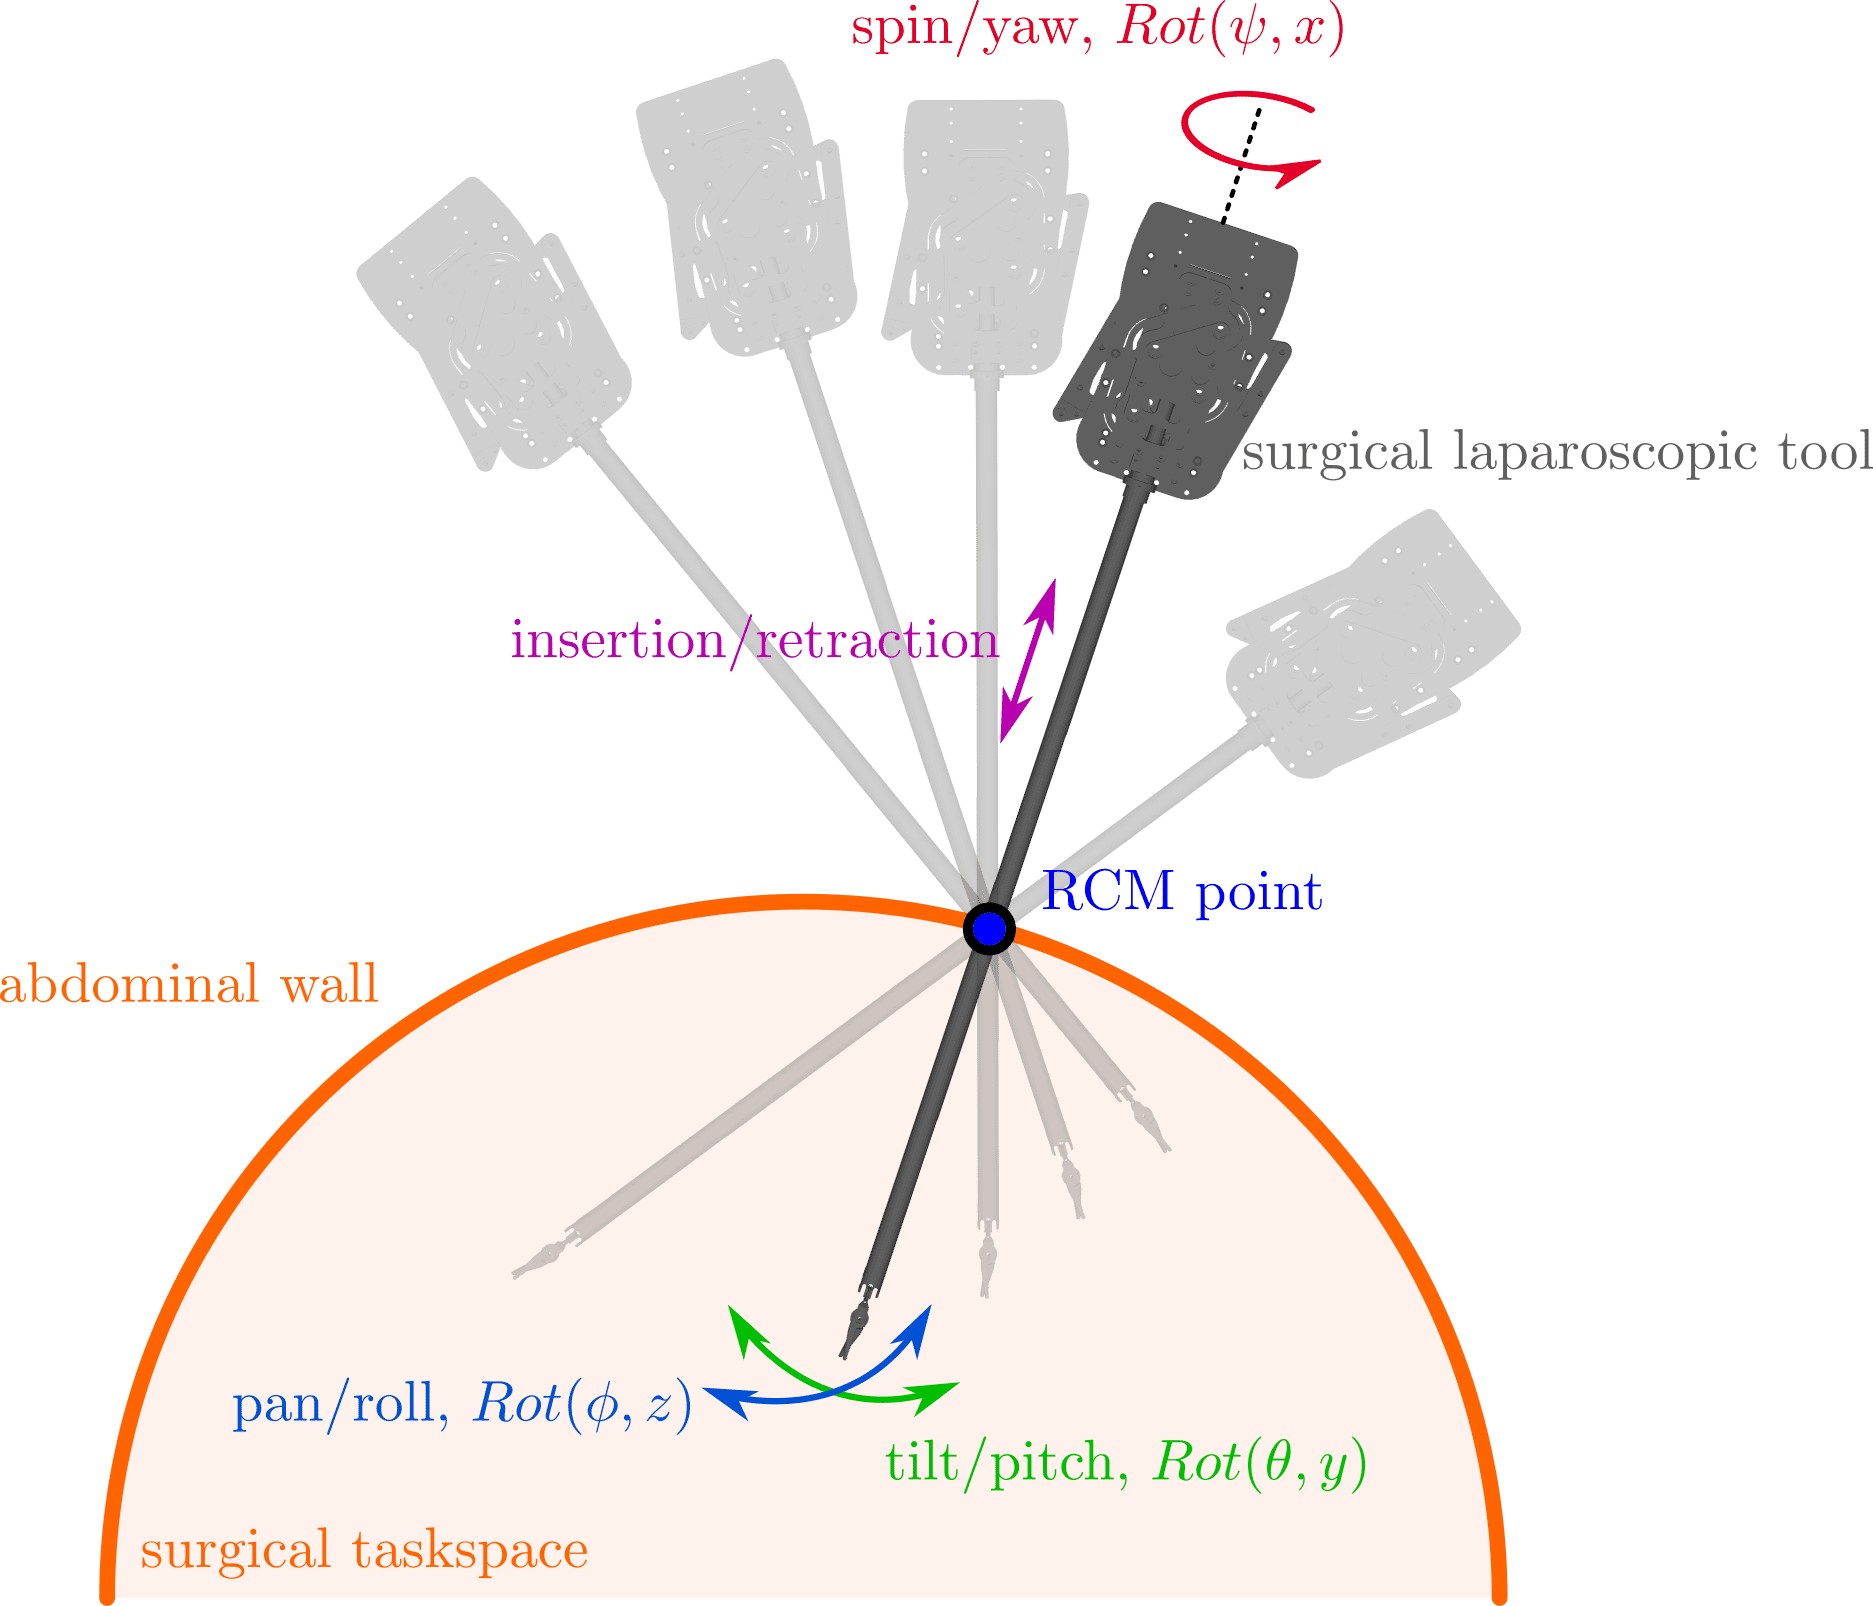
\includegraphics[width=0.8\textwidth]{images/rcm-surgical-tool.png}\\
\caption{Pivoting motion of surgical laparoscopic tool around RCM point.}
\end{figure}

\subsubsection{Elbow-up constraint}
\label{section-elbow-up-constraints}

The IK typically provides 8 different solutions~(see Figures~\ref{iiwa14-solution-configurations} and~\ref{elbow-up-vs-down}). These solutions offer more flexibility to each case, and a different solution is chosen based on the conditions (e.g. previous robot pose) and requirements (e.g. collision avoidance). In this thesis, there are two distinct use cases in terms of choosing a specific robot configuration picking the surgical tools from one table, which does not impose any constraint and the insertion and pivoting of the surgical tool at the mounting dock, which imposes the RCM constraint (see \ref{rcm-subsubsection}) and a constraint to of collision avoidance between the robot arm and the mounting dock.
In the latter use case, in order to satisfy the collision avoidance, all path planning kinematic solutions must be in a elbow-up configuration at all times.

\begin{center}
\begin{figure}[htbp]
\centering
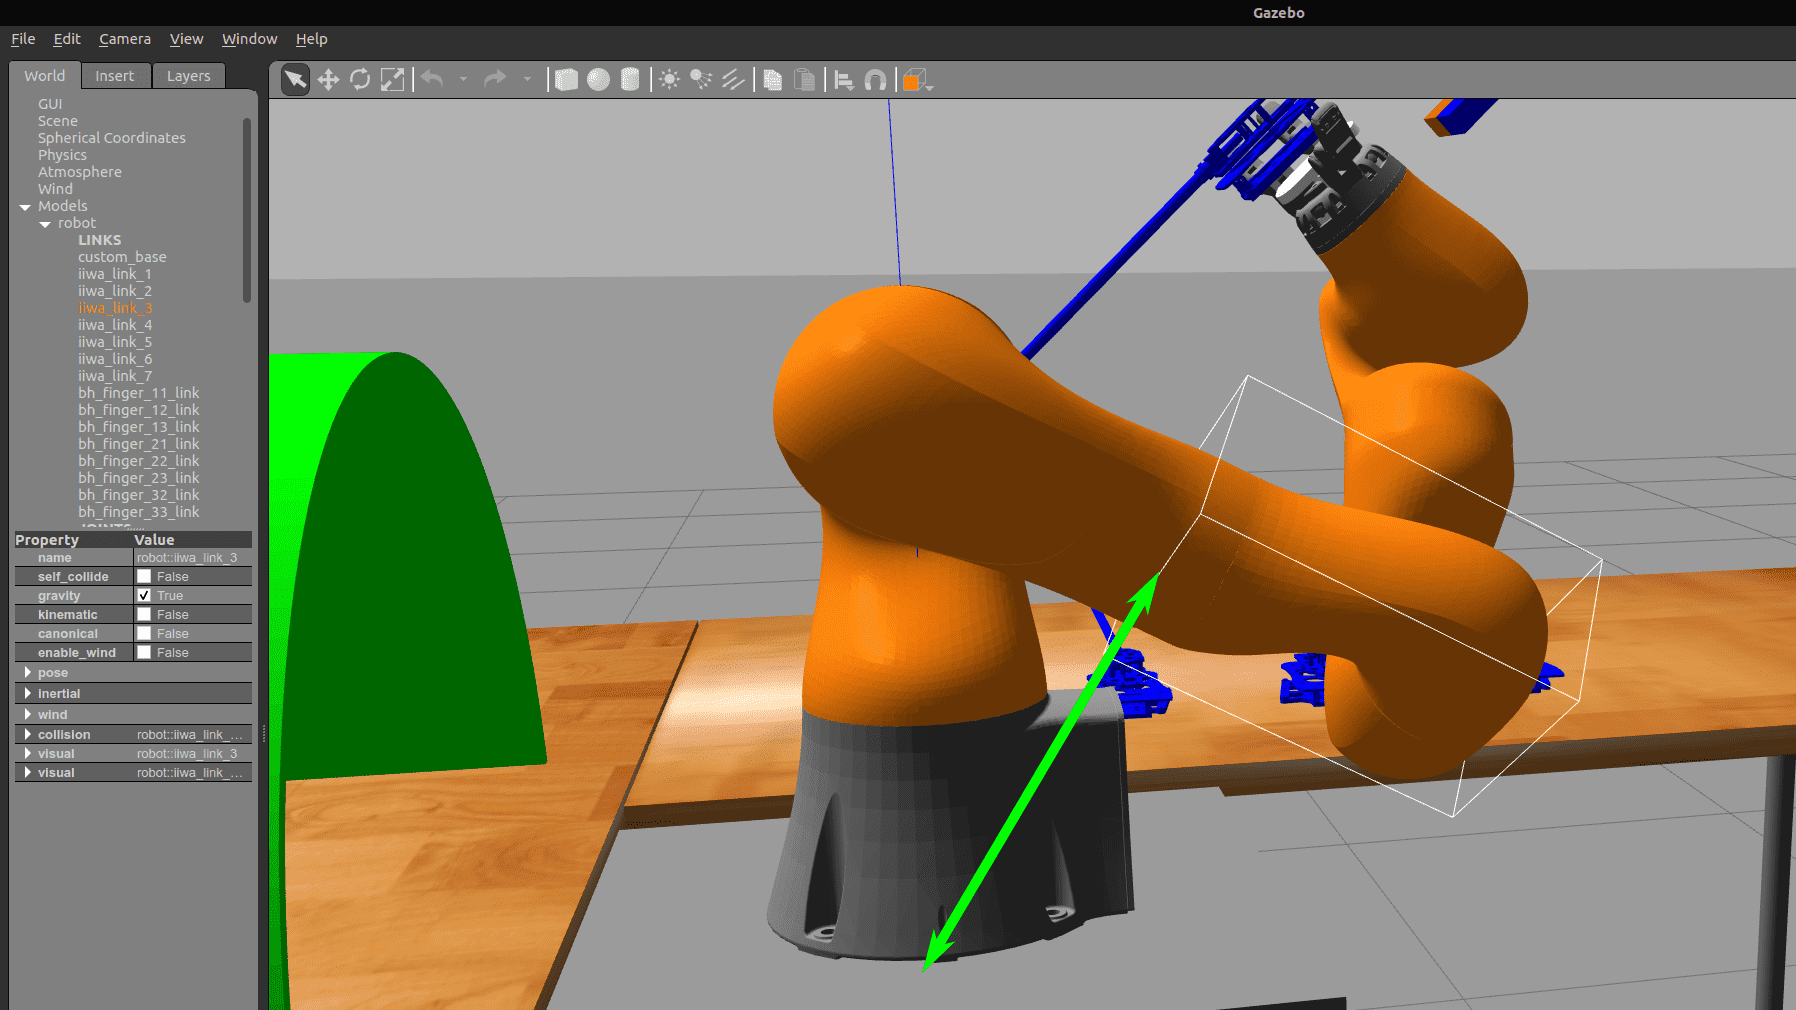
\includegraphics[width=0.8\textwidth]{images/elbow-down.png}\\
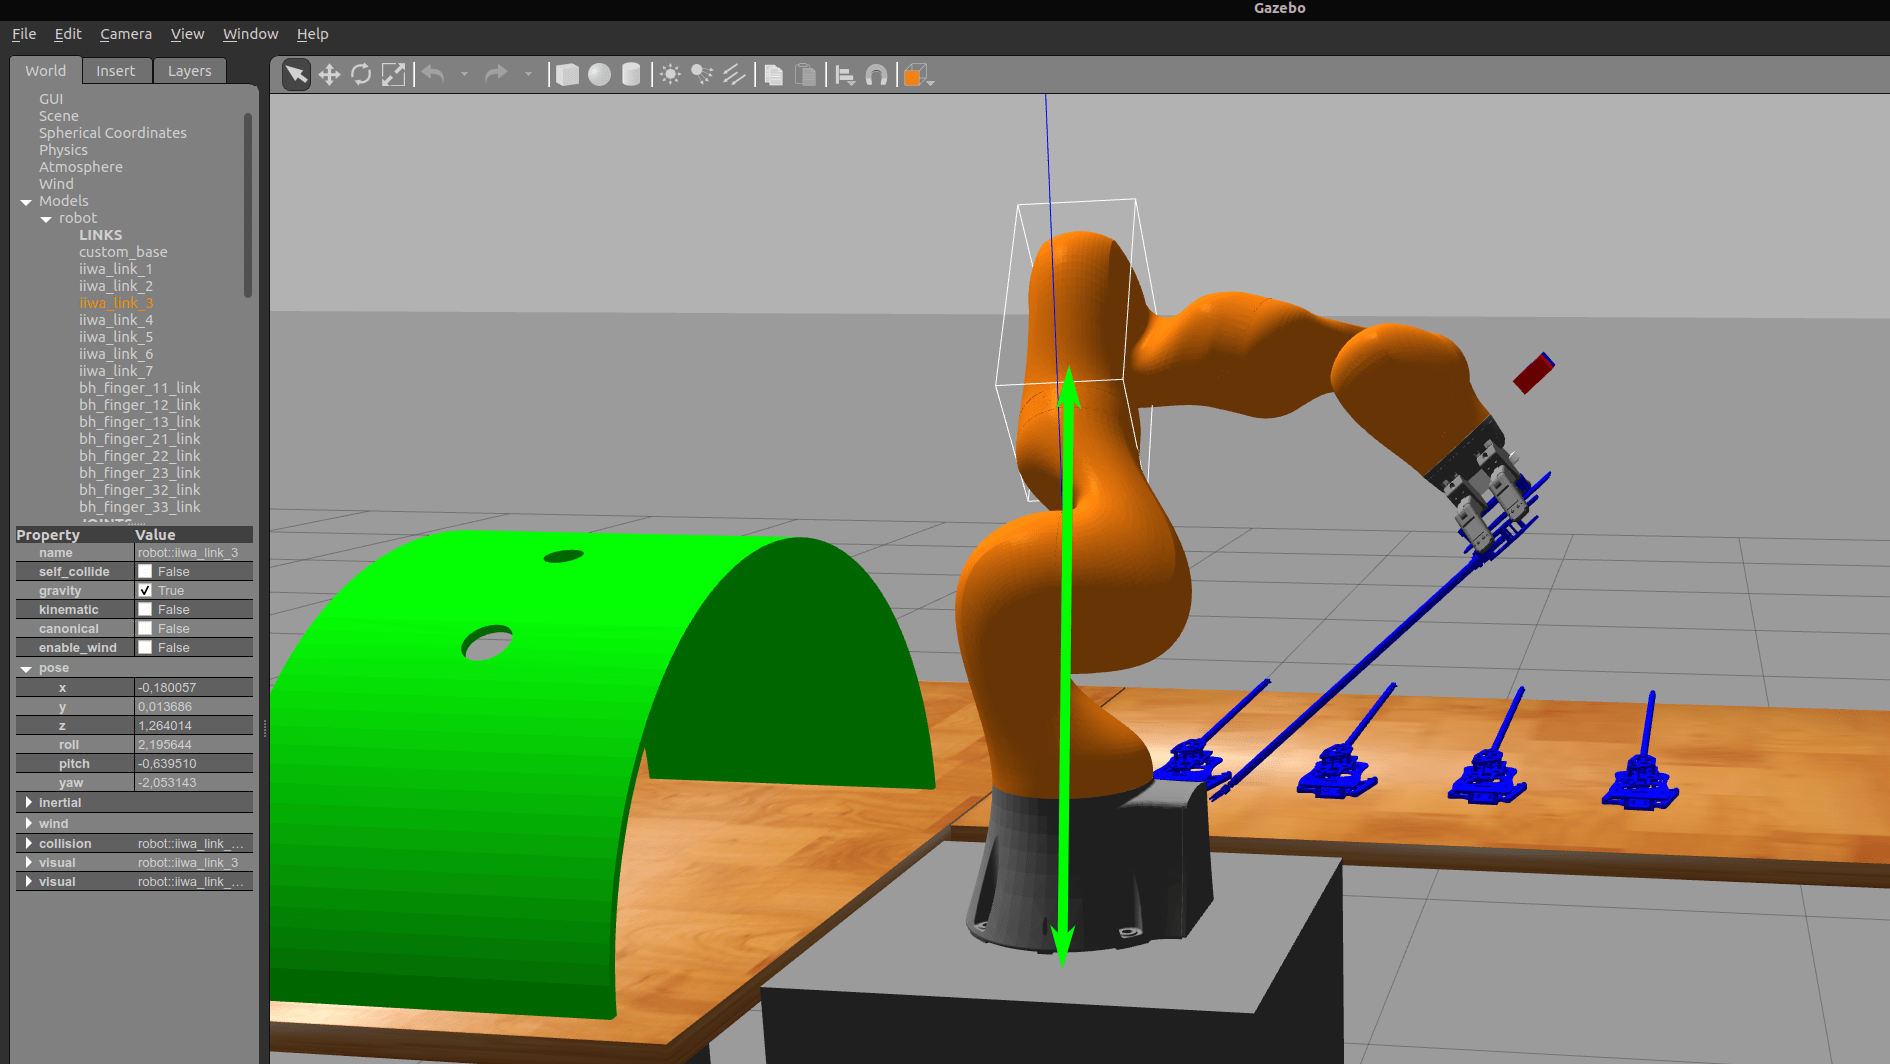
\includegraphics[width=0.8\textwidth]{images/elbow-up.png}\\
\caption{Top: elbow-down solution, bottom: elbow-up solution}
\label{elbow-up-vs-down}
\end{figure}
\end{center}

Observing Figure~\ref{elbow-up-vs-down}, there are two ways to mathematically describe the elbow-up constraint (see Figure~ \ref{elbow-up-constraint-geometry}), either using the distance between the robot base and the 3rd link or by using the relative angle of the base link and the 3rd link. From the iiwa14 specifications, the following calculations are implemented using $d_1 = 360$mm and $d_3 = 420$mm.

\begin{figure}[htbp]
\centering
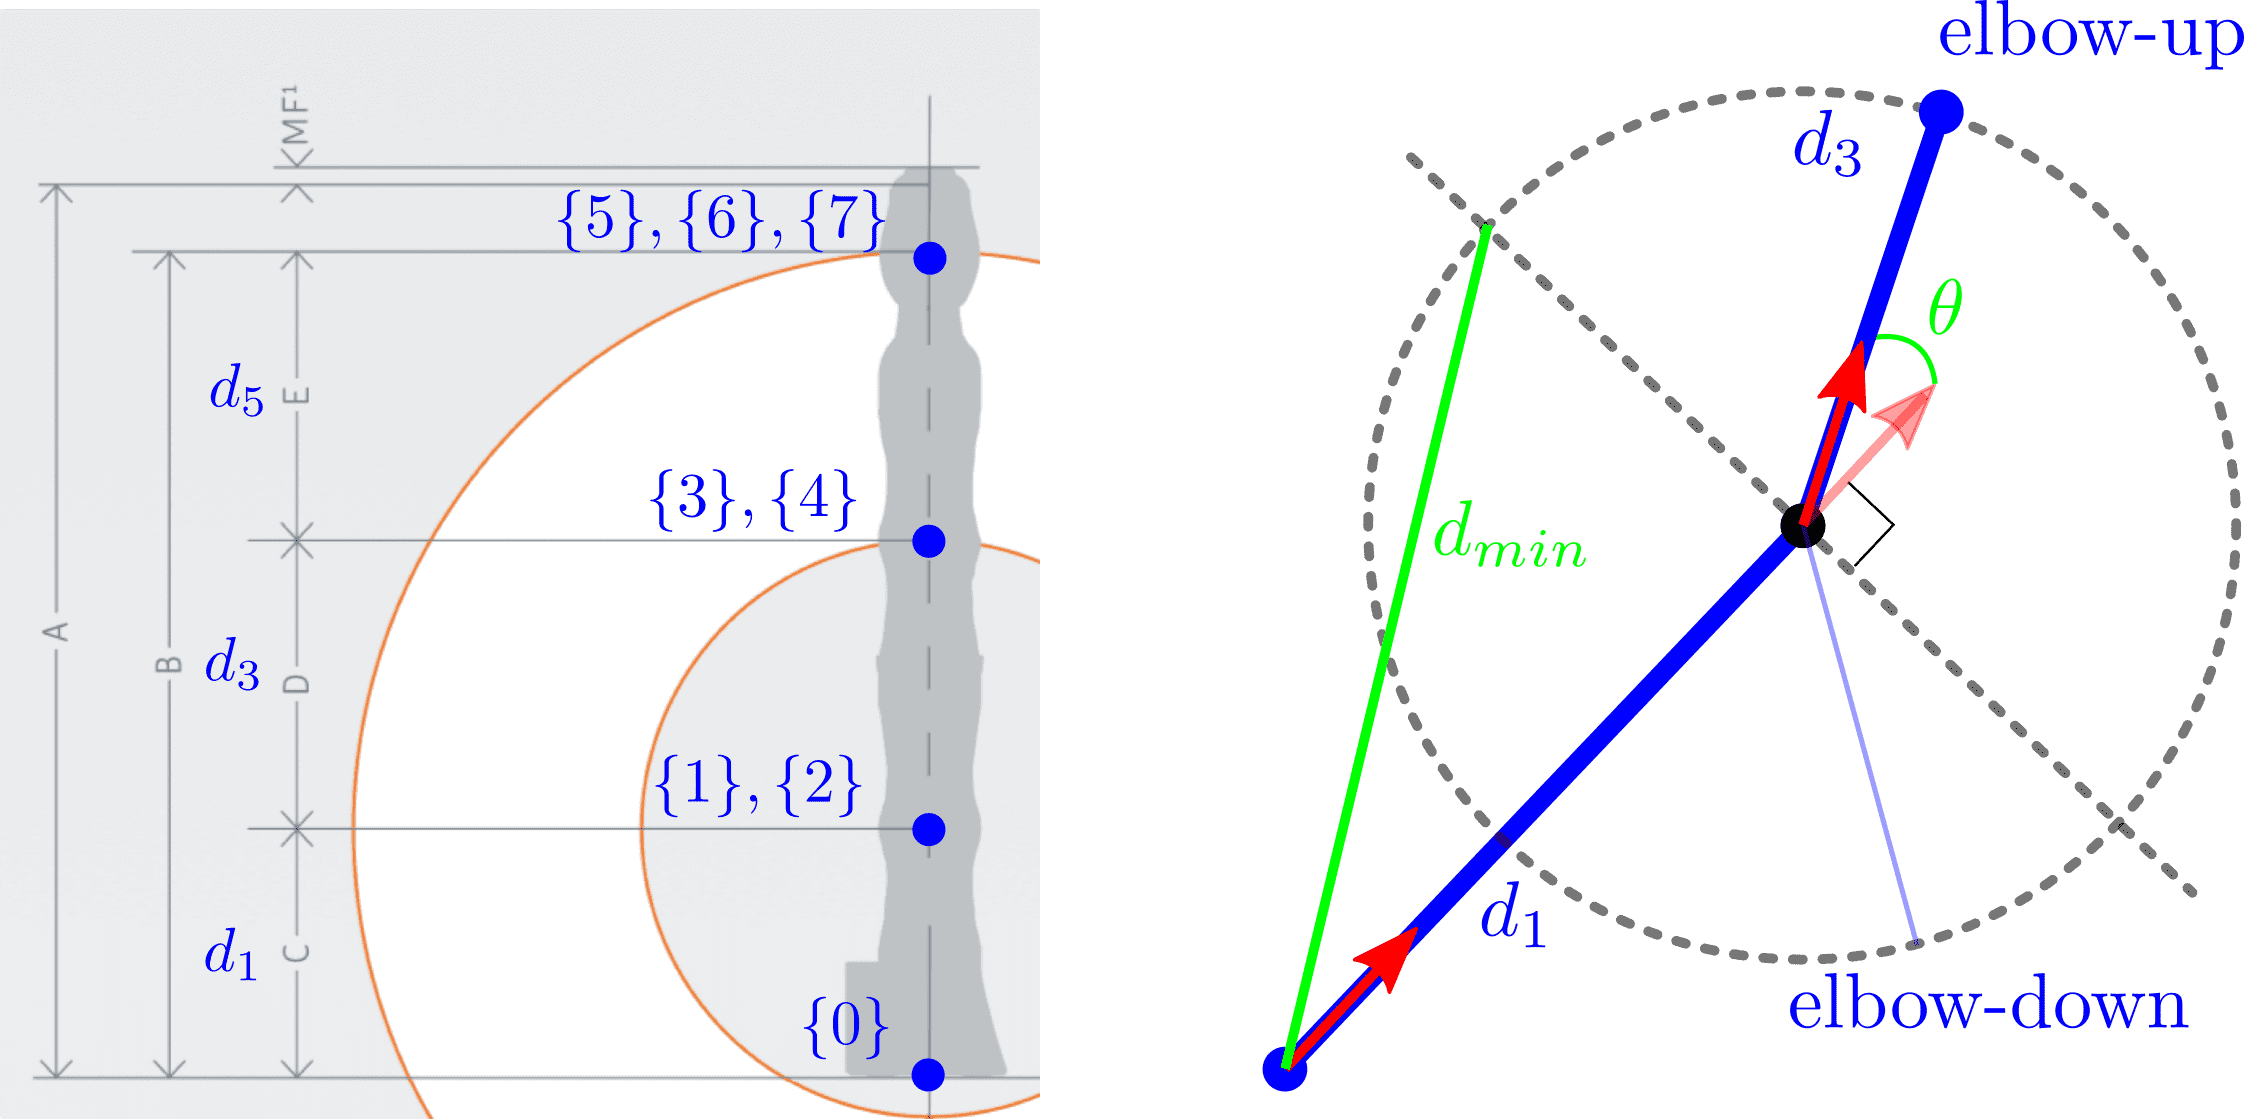
\includegraphics[width=0.8\textwidth]{images/elbow-up-constraint-geometry.png}\\
\caption{Elbow-up constraint description with relative distance or angle between links with lengths $d_1$ and $d_3$}
\label{elbow-up-constraint-geometry}
\end{figure}

The distance constraint is $d_{\min} \leq d \leq d_{\max}$,
%\begin{equation}\label{eq:elbow-up-constraint-distance-inequality}d_{\min} \leq d \leq d_{\max},\end{equation}
where
$d_{\min} = \sqrt{d_1^2 + d_3^2} = 553$mm and $d_{\max} = d_1 + d_3 = 780\mbox{mm}.
$
The distance-based description of the elbow-up constraint is not very convenient, because it can not be easily forward-transformed to a description that uses the robot's forward kinematic transformations and reference frames, 
but it can be easily used after the inverse kinematics solution to check which solutions satisfy this distance constraint. 
The angle-based description can sometimes be more convenient because it directly describes the orientation that the 3rd reference frame must have, with respect to the reference frame of the base. Thus for each orientation 
angle (pitch, yaw, roll) the following constraint must be satisfied 
$-\frac{\pi}{2} \leq θ \leq \frac{\pi}{2}$.
%\begin{equation} \label{eq:elbow-up-constraint-angle-inequality} -\frac{\pi}{2} \leq θ \leq \frac{\pi}{2}. \end{equation}
When the inverse kinematics problem is solved, then some of the solutions may be rejected from the elbow-up constraint after the following calculations. For each solution the forward kinematics up to the 3rd joint must be 
calculated. Note that although the forward kinematics from the universal frame to the end-effector should be the same for all solutions, the same does not hold for the forward kinematic transformations of the intermediate 
links.

\begin{equation}
{}^UT_{tcp} = {}^UT_0  \;\;  {}^0T_3  \;\;   {}^3T_{tcp}
\end{equation}

\begin{equation}
{}^0T_3 = {}^UT_0^{-1}  \;\;  {}^UT_{tcp}  \;\;   {}^3T_{tcp}^{-1}
\end{equation}

Let the calculated ${}^0T_3$ have the following form
\begin{equation}
{}^0T_3 = \begin{bmatrix}
{}^0R_3 & {}^0\mathbf{p}_3 \\
0       & 1 \\
\end{bmatrix}
\end{equation}

then the distance that must satisfy the inequality $d_{\min} \leq d \leq d_{\max}$ is 
\begin{equation}
d = \Vert {}^0\mathbf{p}_3 \Vert
\end{equation}

In a similar way, the angle version of the elbow-up constraint can be used to check if a solution is accepted. Let the orientation matrix ${}^0R_3$ of the calculated pose ${}^0T_3$ have the following form
\begin{equation}
{}^0R_3 = [ {}^0\mathbf{\hat{x}}_3 \quad {}^0\mathbf{\hat{y}}_3 \quad {}^0\mathbf{\hat{z}}_3 ]
\end{equation}

then the angle that must satisfy the inequality $-\frac{\pi}{2} \leq θ \leq \frac{\pi}{2}$ is
\begin{equation}
θ = acos \left( \frac{ {}^0\mathbf{\hat{z}}_3 \cdot {}^0\mathbf{\hat{z}} }{ \Vert {}^0\mathbf{\hat{z}}_3 \Vert  \Vert {}^0\mathbf{\hat{z}} \Vert } \right)
\end{equation}

where ${}^0\mathbf{\hat{z}}$ is the unit vector of the z-axis of the frame $\lbrace 0 \rbrace$ with respect to itself, i.e. ${}^0\mathbf{\hat{z}} = [0, 0, 1]^\top$